\emph{Навчання з підсиленням (Reinforcement learning)} - навчання про те, які дії потрібно приймати залежно від ситуації таким чином, щоб максимізувати \emph{числовий сигнал "винагороди" (reward signal)}. "Учневі" не вказується, які дії потрібно приймати, щоб досягти мети, а натомість дається можливість вибирати з певного набору допустимих дії. В результаті пошуку найкращих дій методом спроб та помилок, досягається оптимальна ``стратегія''.

В загальному випадку, вибрані дії впливають не тільки на винагороду, що слідує безпосередньо після вчинення дії, але й на майбутні ситуації, що, в свою чергу, дає вплив на мабутні винагороди.

Загалом, в навчанні з підсиленням є присутніми дві сутності - агент та середовище. Агент - це все те, на що ми можимо чинити безпосередній вплив. Накриклад, якщо ми маємо робота, то агентом може бути як весь робот, якщо ми здатні безпосередньо керувати поворотом коліс. Або агентом можна визначити лише електромотори, які зумовлюють поворот коліс та їх рух. В останньому випадку, ми безпосередньо можемо впливати тільки на силу струму, що подається на електромотори. На самі ж колеса ми впливаємо опосередковано, тому вони вважаються середовищем, по відношенню до нашого агента.

\begin{figure}[!h]\begin{center}
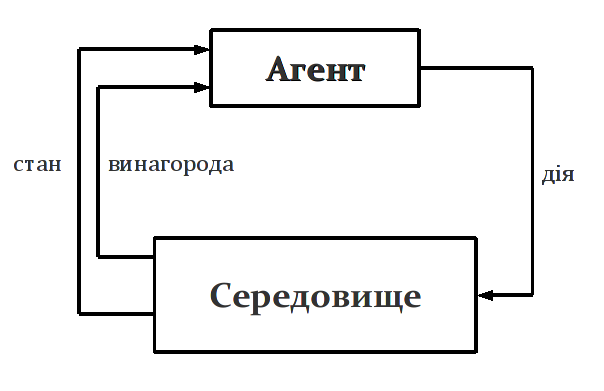
\includegraphics[width=0.7\textwidth]{agent_env_diagram.png}
\caption{Взаємодія агента та середовища в навчанні з підсиленням}
\end{center}\end{figure}

Стан системи - набір параметрів, які задають наші знання (можливо неповні) про оточуючий світ. Це, фактично, наше сприйняття поточної ситуації навколо нас. Наприклад, в випадку автономного керування ТЗ, станом буде інформації про відстань до найближчої перешкоди, відстань до заданої цілі, можливо, поточна швидкість самого ТЗ тощо.

Складовими частинами системи навчання з підсиленнями є:
\begin{itemize}
\item \emph{Стратегія (policy)}, яка визначає те, які дії будуть прийматися залежно від ситуації на даний момент часу. Це фактично є поточний інтелект системи.
\item \emph{Функція винагороди (reward function)}, яка задає скаляр винагороди, який надається системі при здійсенні певної дії в певній ситуації. Глобальною метою є максимізація загальної винагороди, отриманої протягом дії (життя?) системи.
\item \emph{Ціннісна функція (value function)}, яка, на відміну від функції винагороди, задає не те, що є ``корисним'' безпосередньо зараз, а те, що є корисним в більш глобальному значенні, з урахуванням майбутніх станів.
\end{itemize}

В процесі пошуку оптимальної стратегії, виникає так звана проблема компромісу між дослідженням та використанням набутих знань (\emph{exploration-exploitation tradeoff}). Вона полягає в тому, що в процесі пошуку оптимальних дій, потрібно як використовувати вже набуті в процесі попередніх досліджень знання, так і пробувати нові, ще не достатньо дослідженні дії, які могли б покращити поточну стратегію.

Три категорії методів, що застосовуються для розв'язання проблеми навчання з підсиленням:
\begin{itemize}
\item методи динамічного програмування (dynamic programming);
\item методи Монте Карло (Monte Carlo);
\item методи часової різниці (temporal-difference).
\end{itemize}

З цих трьох категорій, методи динамічного програмування дають найкращі результати, проте вони мають суттєві мінуси. Перш за все, для динамічного програмування потрібно знати модель середовища, тобто закони його руху і розвитку, що дуже часто або дуже складно взнати, або в принципі неможливо. Також методам динамічного програмування характерне \emph{``прокляття розмірності'' (``curse of dimensionality'')}, що виявляється в дуже швидкому рості вимог до часу виконання та розміру використовуваної пам'яті з ростом розмірності вектора стану.

Дві інші категорії - це спроба обійти обмеження методів динамічного
програмування - як ``прокляття розмірності'', так і вимог до знання моделі
середовища.
%

\newpage
